\chapter{Návrh}

\setcounter{page}{1}

\section{Uživatelské rozhraní}

Seznam hlasování

\begin{figure}[h]
	\begin{minipage}{0.5\textwidth}
		\centering
		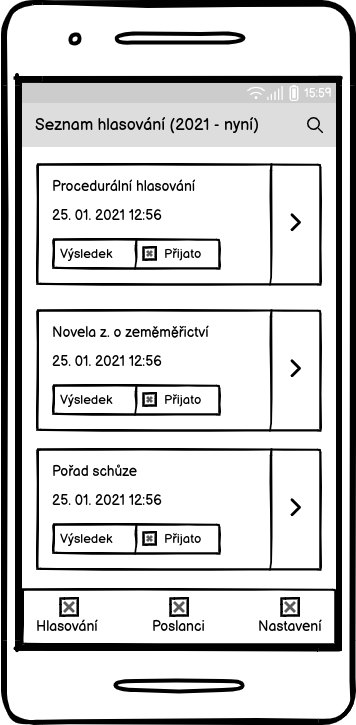
\includegraphics[scale = 0.1]{vote_list.png}
		\caption{Obrazovka pro seznam hlasování}
	\end{minipage}%
	\begin{minipage}{0.5\textwidth}
		\centering
		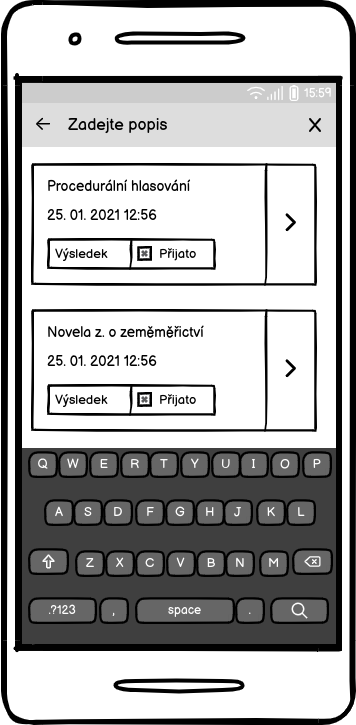
\includegraphics[scale = 0.1]{vote_list_search.png}
		\caption{Obrazovka vyhledávání v seznamu hlasování}
	\end{minipage}
	\caption{Obrazovka pro seznam hlasování}
\end{figure}

Detail hlasování

\begin{figure}[h]
	\begin{minipage}{0.5\textwidth}
		\centering
		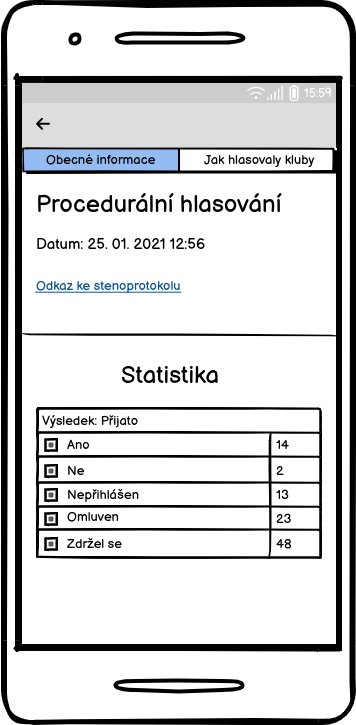
\includegraphics[scale = 0.1]{vote_details_general.png}
		\caption{Obrazovka pro seznam hlasování}
	\end{minipage}%
	\begin{minipage}{0.5\textwidth}
		\centering
		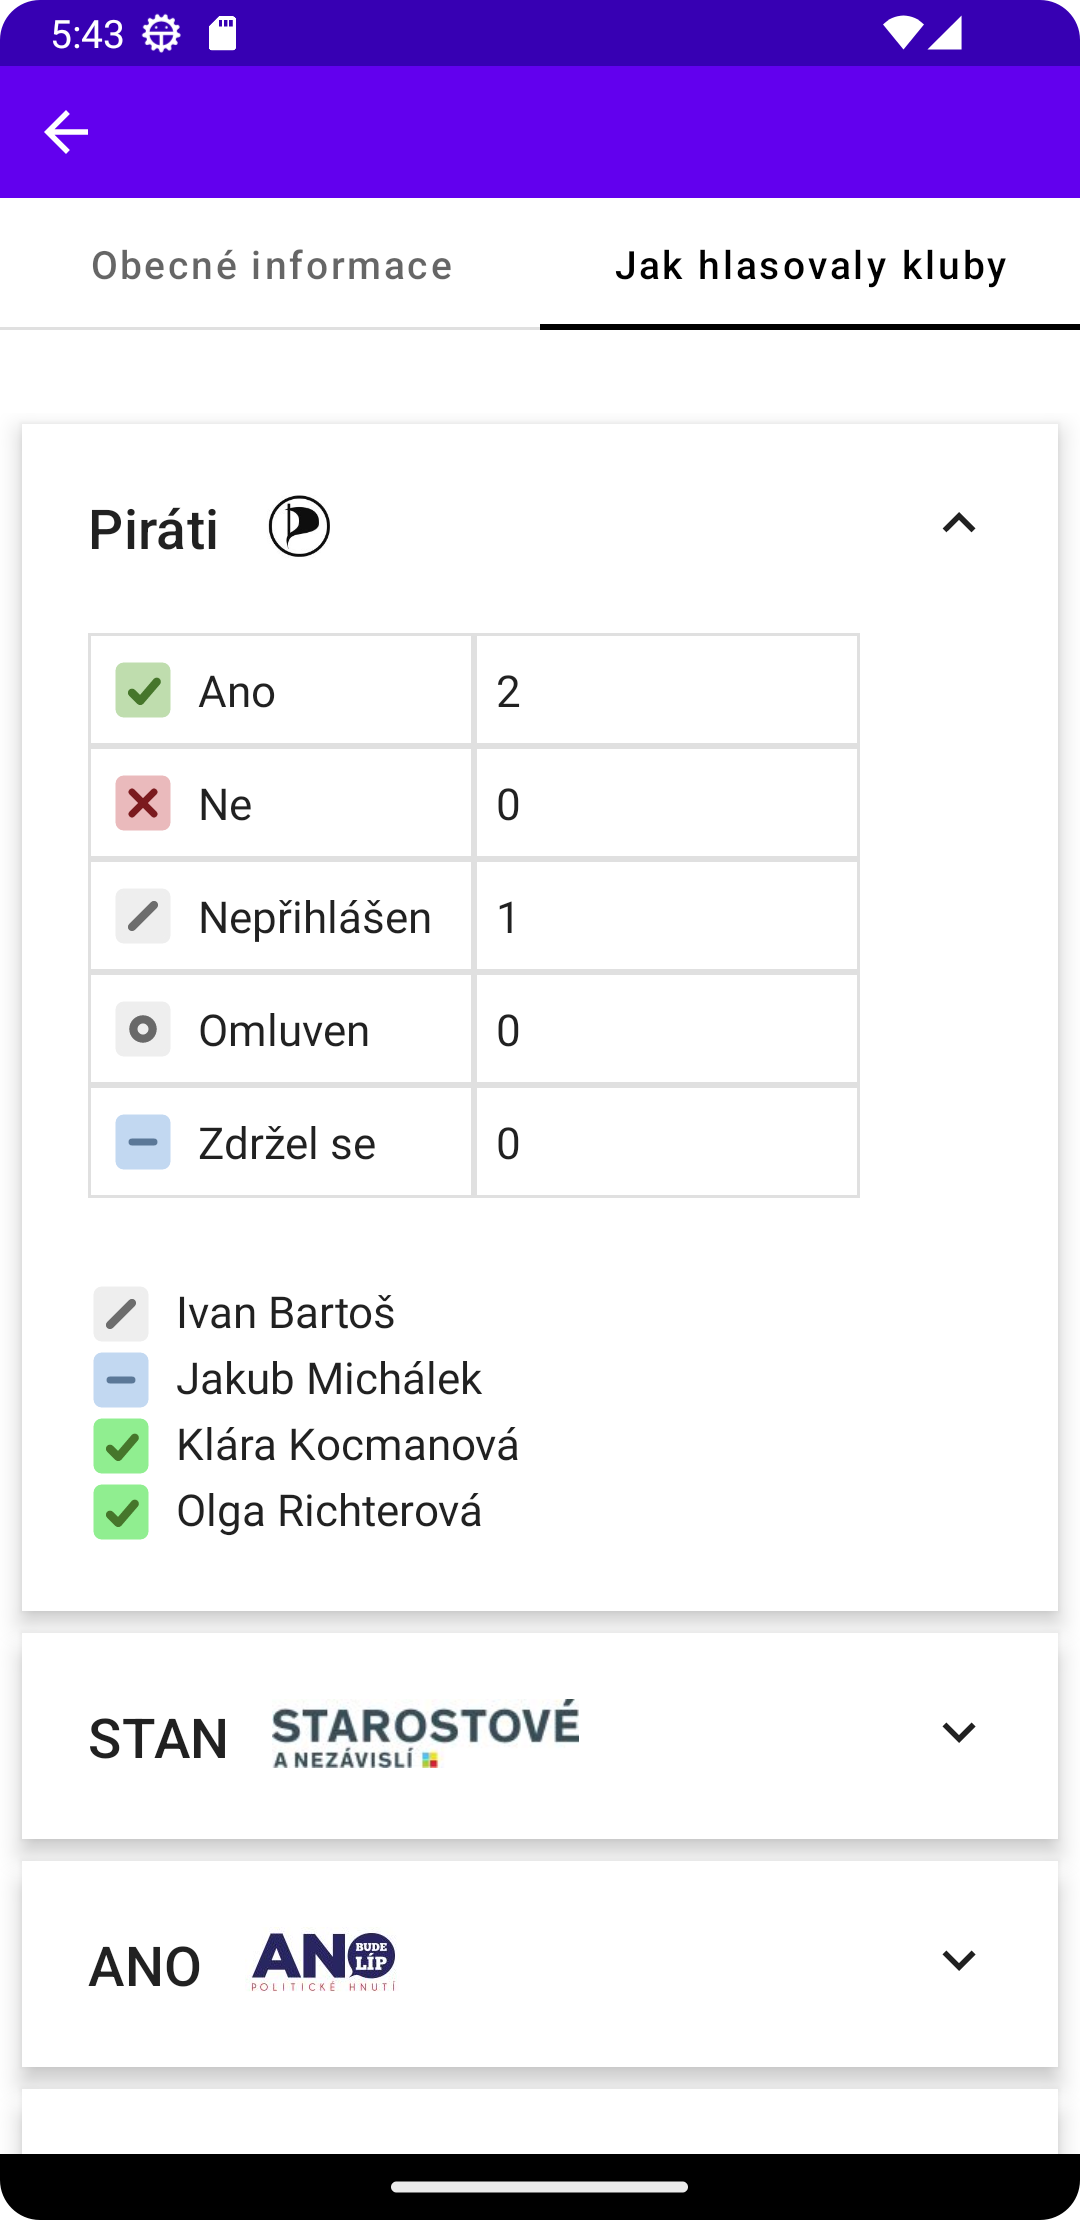
\includegraphics[scale = 0.1]{vote_details_party_opened.png}
		\caption{Obrazovka vyhledávání v seznamu hlasování}
	\end{minipage}
	\caption{Obrazovka pro detail hlasování}
\end{figure}

Seznam poslanců

\begin{figure}[h]
	\begin{minipage}{0.5\textwidth}
		\centering
		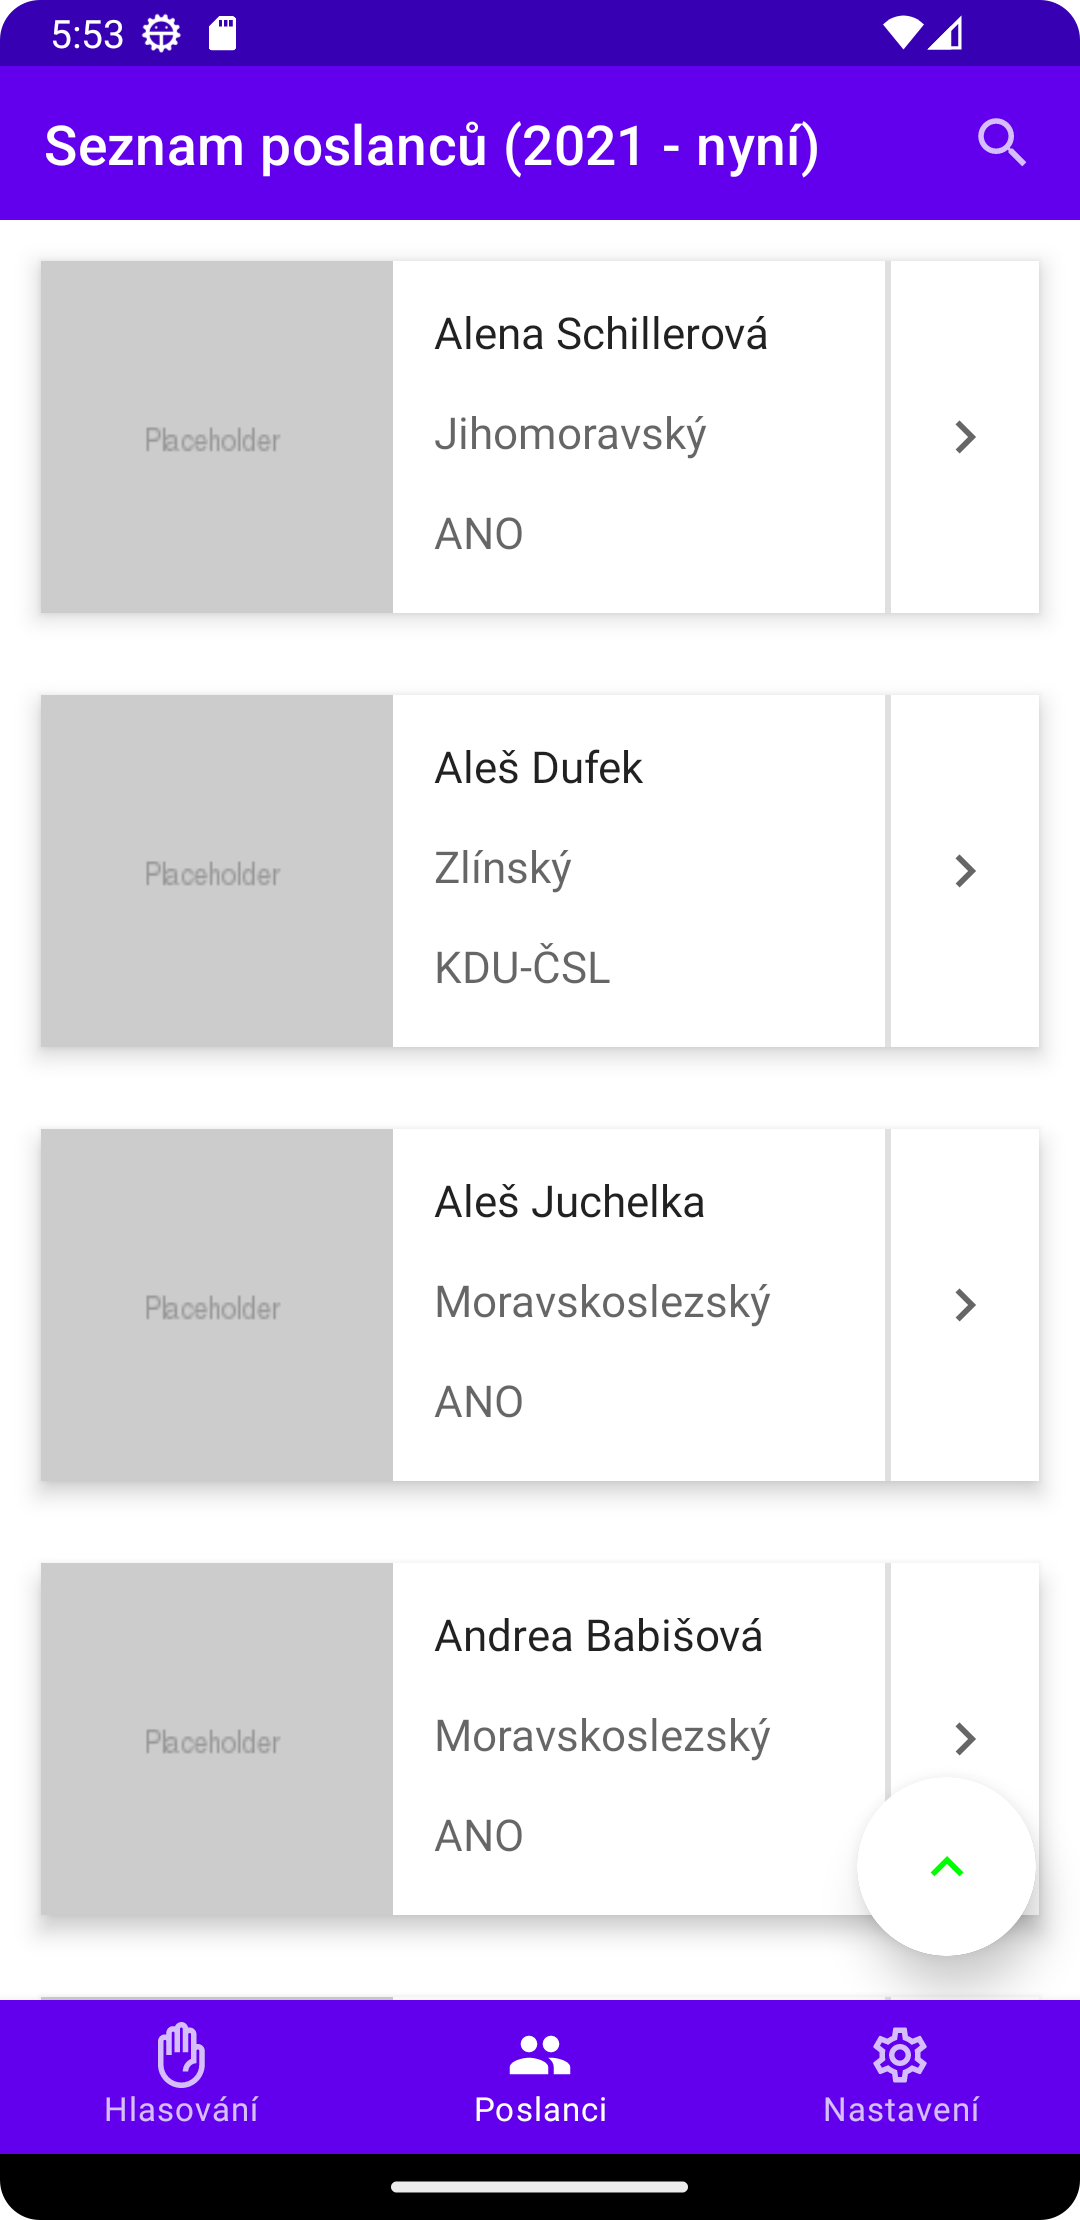
\includegraphics[scale = 0.1]{member_list.png}
		\caption{Obrazovka pro seznam hlasování}
	\end{minipage}%
	\begin{minipage}{0.5\textwidth}
		\centering
		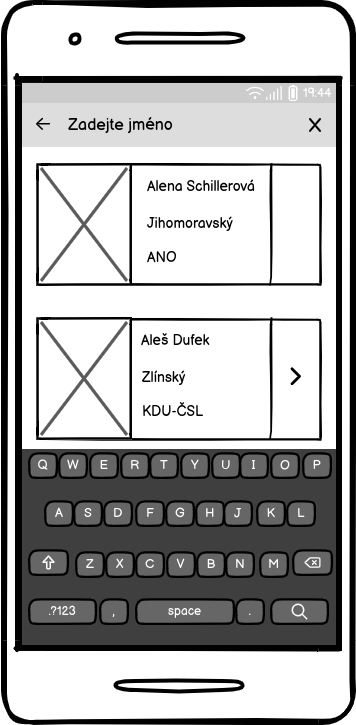
\includegraphics[scale = 0.1]{member_list_search.png}
		\caption{Obrazovka vyhledávání v seznamu hlasování}
	\end{minipage}
	\caption{Obrazovka pro seznam poslanců}
\end{figure}

Detail poslance

\begin{figure}[h]
	\begin{minipage}{0.5\textwidth}
		\centering
		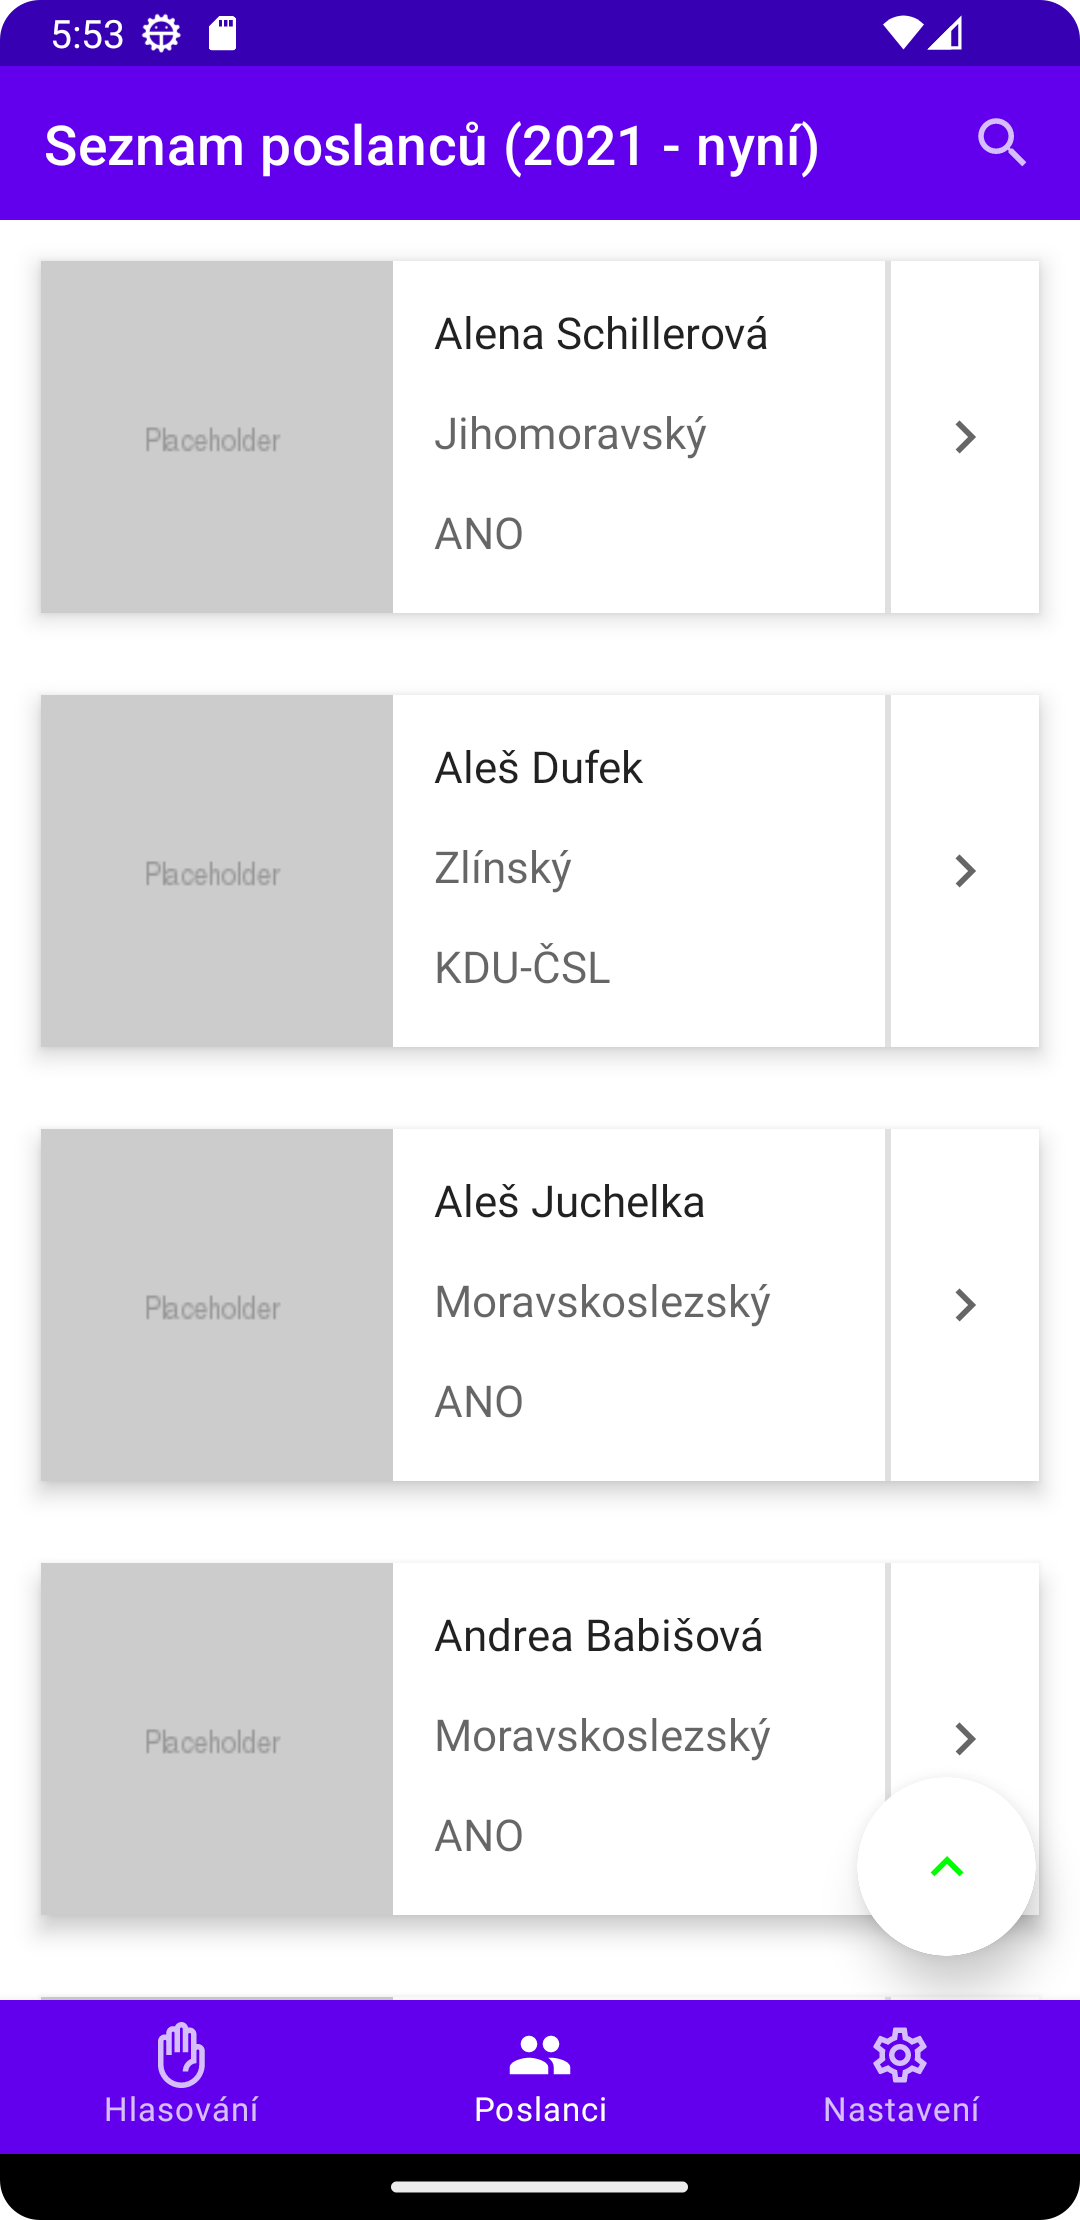
\includegraphics[scale = 0.1]{member_list.png}
		\caption{Obrazovka pro seznam hlasování}
	\end{minipage}%
	\begin{minipage}{0.5\textwidth}
		\centering
		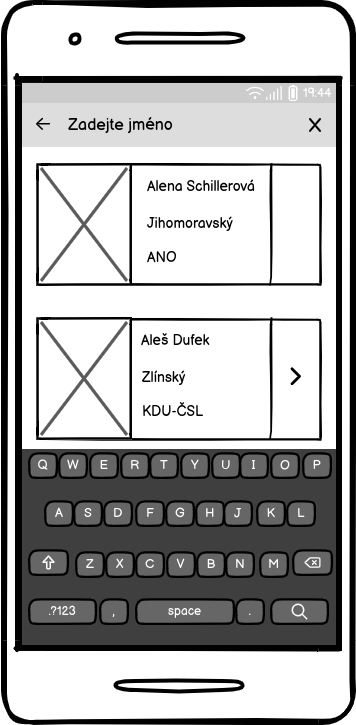
\includegraphics[scale = 0.1]{member_list_search.png}
		\caption{Obrazovka vyhledávání v seznamu hlasování}
	\end{minipage}
	\caption{Obrazovka pro detail poslance}
\end{figure}

Nastavení

\begin{figure}[h]
	\begin{minipage}{0.5\textwidth}
		\centering
		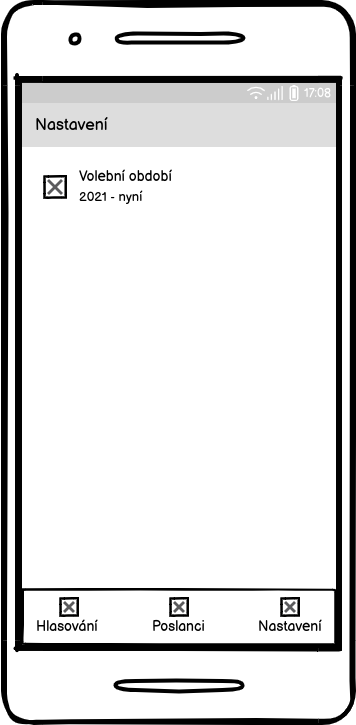
\includegraphics[scale = 0.1]{settings.png}
		\caption{Obrazovka pro seznam hlasování}
	\end{minipage}%
	\begin{minipage}{0.5\textwidth}
		\centering
		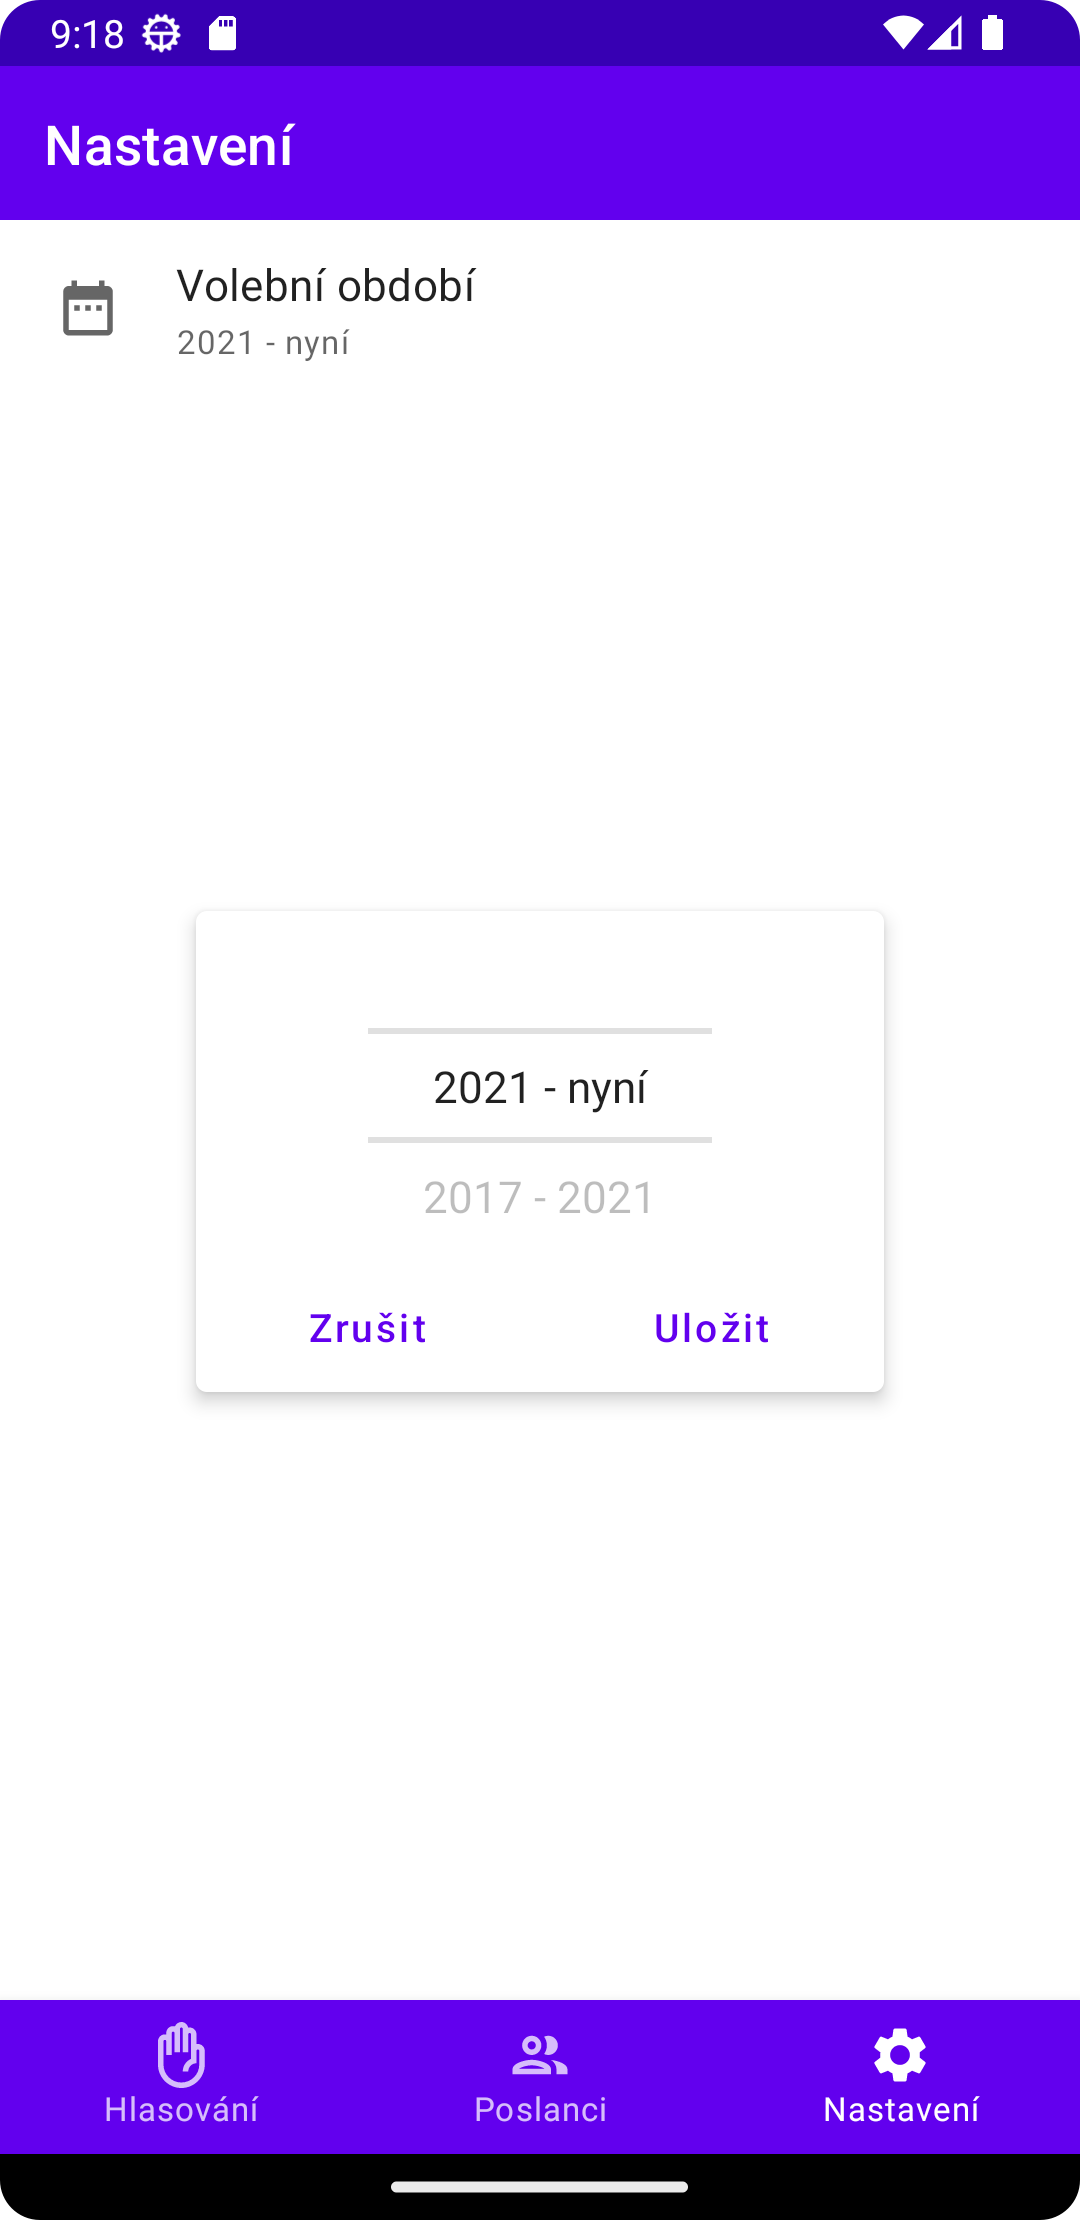
\includegraphics[scale = 0.1]{settings_election_period.png}
		\caption{Obrazovka vyhledávání v seznamu hlasování}
	\end{minipage}
	\caption{Obrazovka pro nastavení}
\end{figure}

\section{REST API}

Stav aplikace

\begin{lstlisting}[]
GET /api/app
\end{lstlisting}

\begin{lstlisting}[language=json,firstnumber=1,tabsize=2]
{
	"menu": {
		"id": "file",
		"value": "File",
		"popup": {
			"menuitem": [
				{"value": "New", "onclick": "CreateNewDoc()"},
				{"value": "Open", "onclick": "OpenDoc()"},
				{"value": "Close", "onclick": "CloseDoc()"}
			]
		}
	}
}
\end{lstlisting}

Seznam hlasování

\begin{lstlisting}[]
GET /api/vote
\end{lstlisting}

\begin{lstlisting}[language=json,firstnumber=1,tabsize=2]
[
	{
		"id": 1,
		"date_time": "16. 12. 2022 13:29",
		"description": "Hlasovani 1",
		"result": "A"
	},
	{
		"id": 2,
		"date_time": "16. 12. 2022 13:26",
		"description": "Hlasovani 2",
		"result": "A"
	},
]
\end{lstlisting}

Detail hlasování

\begin{lstlisting}[]
GET /api/vote/1
\end{lstlisting}

\begin{lstlisting}[language=json,firstnumber=1,tabsize=2]
{
	"id": 1,
	"date_time": "16. 12. 2022 13:29",
	"description": "Hlasovani 1,
	"result": "A",
	"steno_protocol_url": "http://www.psp.cz/eknih/2021ps/stenprot/048schuz/s048109.htm#h76",
	"yes_count": 100,
	"no_count": 0,
	"logged_off_count": 64,
	"excused_count": 0,
	"refrained_count": 36,
	"election_year": 0
}
\end{lstlisting}

Jak hlasovaly kluby a jejich členové v daném hlasování

\begin{lstlisting}[]
GET /api//party/vote/1
\end{lstlisting}

\begin{lstlisting}[language=json,firstnumber=1,tabsize=2]
[
	{
		"party_name": "Nazev klubu",
		"logo_url": "https://www.psp.cz/pics/klub/l-cps.jpg",
		"vote_id": 1,
		"party_results": {
			"yes_count": 2,
			"no_count": 0,
			"logged_off_count": 1,
			"excused_count": 0,
			"refrained_count": 0
		},
		"member_results": [
		{
			"member_name": "Poslanec 1",
			"vote_result": "@"
		},
		{
			"member_name": "Poslanec 2",
			"vote_result": "C"
		},
		{
			"member_name": "Poslanec 3",
			"vote_result": "A"
		},
		{
			"member_name": "Poslanec 4",
			"vote_result": "A"
		}
		]
	}
]
\end{lstlisting}

Seznam poslanců

\begin{lstlisting}[]
GET /api/member
\end{lstlisting}

\begin{lstlisting}[language=json,firstnumber=1,tabsize=2]
[
	{
		"id": 1,
		"name": "Poslanec 1",
		"party": "ANO",
		"photo_url": "https://www.psp.cz/eknih/cdrom/2021ps/eknih/2021ps/poslanci/i6474.jpg",
		"election_region": "Volebni kraj 1",
		"election_year": 2021
	},
	{
		"id": 2,
		"name": "Poslanec 2",
		"party": "ODS",
		"photo_url": "https://www.psp.cz/eknih/cdrom/2021ps/eknih/2021ps/poslanci/i6804.jpg",
		"election_region": "Volebni kraj 2",
		"election_year": 2021
	},
]
\end{lstlisting}

Detail poslance

\begin{lstlisting}[]
GET /api/member/1
\end{lstlisting}

\begin{lstlisting}[language=json,firstnumber=1,tabsize=2]
{
	"id": 1,
	"name": "Poslanec 1",
	"gender": "M",
	"party": "Poslanecky klub",
	"member_from": "12. 10. 2021",
	"member_to": null,
	"date_of_birth": "25. 09. 1970",
	"election_region": "Volebni kraj 1",
	"photo_url": "https://www.psp.cz/eknih/cdrom/2021ps/eknih/2021ps/poslanci/i6474.jpg",
	"election_year": 2021
}
\end{lstlisting}

Jak hlasoval poslanec

\begin{lstlisting}
	GET /api/member/1/vote
\end{lstlisting}

\begin{lstlisting}[language=json,firstnumber=1,tabsize=2]
[
	{
		"vote": {
			"id": 1,
			"date_time": "16. 12. 2022 13:29",
			"description": "Hlasovani 1",
			"result": "A"
		},
		"how_member_voted": "@"
	},
	{
		"vote": {
			"id": 2,
			"date_time": "16. 12. 2022 13:26",
			"description": "Hlasovani 2",
			"result": "A"
		},
		"how_member_voted": "@"
	}
]
\end{lstlisting}

\section{Databázové datové struktury}

Struktura agency.

\begin{table}[!h]\centering
	\caption[Struktura agency]{Struktura agency}\label{table:agency}
	\begin{tabular}{|l|l|p{6cm}|}\hline
		Název	& Typ	& Popis	\tabularnewline \hline \hline
		\texttt{id}		& \texttt{int}	& identifikátor orgánu		\tabularnewline \hline
		\texttt{abbreviation}		& \texttt{varchar(255)}	& zkratka názvu orgánu		\tabularnewline \hline
		\texttt{end\textunderscore date}		& \texttt{date(255)}	& datum zániku orgánu		\tabularnewline \hline
		\texttt{name}		& \texttt{varchar(255)}	& název orgánu		\tabularnewline \hline
		\texttt{start\textunderscore date}		& \texttt{date}	& datum založení orgánu		\tabularnewline \hline
		\texttt{type\textunderscore id}		& \texttt{int}	& identifikátor typu orgánu 		\tabularnewline \hline
	\end{tabular}
\end{table}

Struktura agency\textunderscore type.

\begin{table}[!h]\centering
	\caption[Struktura agency\textunderscore type]{Struktura agency\textunderscore type}\label{table:agency_type}
	\begin{tabular}{|l|l|p{6cm}|}\hline
		Název	& Typ	& Popis	\tabularnewline \hline \hline
		\texttt{id}		& \texttt{int}	& identifikátor typu orgánu		\tabularnewline \hline
		\texttt{name}		& \texttt{varchar(512)}	& název typu orgánu \tabularnewline \hline
		\texttt{superior\textunderscore agency\textunderscore type\textunderscore id}		& \texttt{int}	& identifikátor nadřazeného typu orgánu \tabularnewline \hline
	\end{tabular}
\end{table}

Struktura excuse.

\begin{table}[!h]\centering
	\caption[Struktura excuse]{Struktura excuse}\label{table:excuse}
	\begin{tabular}{|l|l|p{6cm}|}\hline
		Název	& Typ	& Popis	\tabularnewline \hline \hline
		\texttt{member\textunderscore id}		& \texttt{int}	& identifikátor poslance, který je omluven		\tabularnewline \hline
		\texttt{date} & \texttt{date}	& datum, kdy je poslanec omluven \tabularnewline \hline
		\texttt{start\textunderscore time}		& \texttt{time}	& čas, od kterého byl poslanec omluven \tabularnewline \hline
		\texttt{end\textunderscore time}		& \texttt{time}	& čas, do kterého byl poslanec omluven \tabularnewline \hline
		\texttt{election\textunderscore year}		& \texttt{int}	& první rok volebního období \tabularnewline \hline
	\end{tabular}
\end{table}

Struktura member.

\begin{table}[!h]\centering
	\caption[Struktura member]{Struktura member}\label{table:member}
	\begin{tabular}{|l|l|p{6cm}|}\hline
		Název	& Typ	& Popis	\tabularnewline \hline \hline
		\texttt{id}		& \texttt{int}	& identifikátor poslance, který je omluven		\tabularnewline \hline
		\texttt{date\textunderscore of\textunderscore birth} & \texttt{date}	& datum narození \tabularnewline \hline
		\texttt{election\textunderscore region}		& \texttt{varchar(255)}	& volební kraj \tabularnewline \hline
		\texttt{election\textunderscore year}		& \texttt{int}	& první rok volebního období \tabularnewline \hline
		\texttt{gender}		& \texttt{varchar(255)}	& pohlaví \tabularnewline \hline
		\texttt{member\textunderscore from} & \texttt{date} & datum začátku členství \tabularnewline \hline
		\texttt{member\textunderscore to} & \texttt{date} & datum konce členství \tabularnewline \hline
		\texttt{name} & \texttt{varchar(255)} & jméno \tabularnewline \hline
		\texttt{person\textunderscore id} & \texttt{int} & identifikátor osoby \tabularnewline \hline
		\texttt{photo\textunderscore url} & \texttt{varchar(255)} & URL profilové fotky \tabularnewline \hline
		\texttt{party\textunderscore election\textunderscore year} & \texttt{int} & první rok volebního období \tabularnewline \hline
		\texttt{party\textunderscore party\textunderscore id} & \texttt{int} & identifikíátor poslaneckého klubu, jehož je členem \tabularnewline \hline
	\end{tabular}
\end{table}

Struktura member\textunderscore vote.

\begin{table}[!h]\centering
	\caption[Struktura member\textunderscore vote]{Struktura member\textunderscore vote}\label{table:membe_vote}
	\begin{tabular}{|l|l|p{6cm}|}\hline
		Název	& Typ	& Popis	\tabularnewline \hline \hline
		\texttt{result}		& \texttt{varchar(255)}	& jak hlasoval poslanec\tabularnewline \hline
		\texttt{member\textunderscore id}		& \texttt{int}	& jak identifikátor poslance\tabularnewline \hline
		\texttt{vote\textunderscore id}		& \texttt{int}	& identifikátor hlasování\tabularnewline \hline
	\end{tabular}
\end{table}

Struktura membership.

\begin{table}[!h]\centering
	\caption[Struktura membership]{Struktura membership}\label{table:membership}
	\begin{tabular}{|l|l|p{6cm}|}\hline
		Název	& Typ	& Popis	\tabularnewline \hline \hline
		\texttt{end\textunderscore date}		& \texttt{datetime}	& datum a čas konce zařazení\tabularnewline \hline
		\texttt{agency\textunderscore id}		& \texttt{int}	& identifikátor orgánu\tabularnewline \hline
		\texttt{person\textunderscore id}		& \texttt{int}	& identifikátor osoby \tabularnewline \hline
		\texttt{start\textunderscore date}		& \texttt{datetime}	& datum a čas začátku zařazení \tabularnewline \hline
	\end{tabular}
\end{table}

Struktura party.

\begin{table}[!h]\centering
	\caption[Struktura party]{Struktura party}\label{table:party}
	\begin{tabular}{|l|l|p{6cm}|}\hline
		Název	& Typ	& Popis	\tabularnewline \hline \hline
		\texttt{abbreviation} & \texttt{varchar(255)} & zkratka pro název klubu\tabularnewline \hline
		\texttt{name} & \texttt{varchar(255)}	& název klubu\tabularnewline \hline
		\texttt{election\textunderscore year}		& \texttt{int}	& první rok volebního období \tabularnewline \hline
		\texttt{party\textunderscore id}		& \texttt{int}	& identifikátor klubu \tabularnewline \hline
	\end{tabular}
\end{table}

Struktura vote.

\begin{table}[!h]\centering
	\caption[Struktura vote]{Struktura vote}\label{table:vote}
	\begin{tabular}{|l|l|p{6cm}|}\hline
		Název	& Typ	& Popis	\tabularnewline \hline \hline
		\texttt{date\textunderscore time} & \texttt{datetime} & datum a čas hlasování\tabularnewline \hline
		\texttt{description} & \texttt{varchar(255)}	& popis hlasování\tabularnewline \hline
		\texttt{election\textunderscore year}		& \texttt{int}	& první rok volebního období \tabularnewline \hline
		\texttt{excused\textunderscore count}		& \texttt{int}	& počet omluvených \tabularnewline \hline
		\texttt{logged\textunderscore off\textunderscore count}		& \texttt{int}	& počet nepřihlášených \tabularnewline \hline
		\texttt{meeting\textunderscore number}		& \texttt{int}	& bod hlasování \tabularnewline \hline
		\texttt{no\textunderscore count}		& \texttt{int}	& počet hlasování proti \tabularnewline \hline
		\texttt{refrained\textunderscore count}		& \texttt{int}	& počet zdržených \tabularnewline \hline
		\texttt{result}		& \texttt{varchar(255)}	& výsledek hlasování \tabularnewline \hline
		\texttt{steno\textunderscore protocol\textunderscore url}		& \texttt{varchar(255)}	& stenoprotokol \tabularnewline \hline
		\texttt{yes\textunderscore count}		& \texttt{int}	& počet hlasování pro \tabularnewline \hline
		\texttt{number}		& \texttt{int}	& číslo hlasování \tabularnewline \hline
		\texttt{id}		& \texttt{int}	& identifikátor hlasování \tabularnewline \hline
	\end{tabular}
\end{table}